% Created with jtex v.1.0.20
\documentclass{article}
\usepackage{arxiv}

\usepackage[utf8]{inputenc} % allow utf-8 input
\usepackage[T1]{fontenc}    % use 8-bit T1 fonts
\usepackage{hyperref}       % hyperlinks
\usepackage{url}            % simple URL typesetting
\usepackage{datetime}       % show dates in the title block
\usepackage{booktabs}       % professional-quality tables
\usepackage{amsfonts}       % blackboard math symbols
\usepackage{nicefrac}       % compact symbols for 1/2, etc.
\usepackage{microtype}      % microtypography
\usepackage{graphicx}
\usepackage{natbib}
\usepackage{doi}
\usepackage{xcolor}

%%%%%%%%%%%%%%%%%%%%%%%%%%%%%%%%%%%%%%%%%%%%%%%%%%
%%%%%%%%%%%%%%%%%%%%  imports  %%%%%%%%%%%%%%%%%%%
\usepackage{amsmath}
%%%%%%%%%%%%%%%%%%%%%%%%%%%%%%%%%%%%%%%%%%%%%%%%%%


\hypersetup{colorlinks = true,
linkcolor = purple,
urlcolor  = blue,
citecolor = cyan,
anchorcolor = black}

\title{Research Paper}

\newdate{articleDate}{18}{11}{2024}
\date{\displaydate{articleDate}}

\makeatletter
\let\@fnsymbol\@arabic
\makeatother

\author{Yasmine Mettawa\\
}

% Uncomment to override  the `A preprint' in the header
\renewcommand{\headeright}{}
\renewcommand{\undertitle}{}
\renewcommand{\shorttitle}{}

%% Add PDF metadata to help others organize their library
%% Once the PDF is generated, you can check the metadata with
%% $ pdfinfo template.pdf
\hypersetup{
pdftitle={\@title},
pdfsubject={},
pdfauthor={\@author},
pdfkeywords={},
addtopdfcreator={Written in Curvenote}
}

\begin{document}
\maketitle



\part{Content}

\chapter{Abstract}

This paper explores how labor force participation rates in the United States from 1948 to 2020 are influenced by political party governance at the state and national level. Using a Weighted Least Squared (WLS) regression, the study analyzes changes in labor force participation, comparing states with Republican governors (treatment group) to those with Democratic governors (control group), as well as an Ordinary Least Squared (OLS) regression analyzing changes in labor force participation against the political party of the president, either Republican (treatment group) or Democratic (control group). The findings suggest that on both the national and state level political party leadership does not correlate with increased labor force participation. Therefore, it can not be concluded that there exists a direct relationship.

\chapter{Introduction}

The research question being explored is: ``How does the labor force participation rate from the 1953 until 2020 in the United States vary with political party governance, as well as broader policies implemented by said parties?'' The topic seeks to consider factors that lead to changes in labor force participation rates particularly in terms of policy. If there exists a statistically significant relationship policy tendencies of said party will be explored to isolate particular ones with a significant effect.

The period of 1953 through 2020 will be used for national statistics on labor force participation rate, however for state wide statistics the period observed will be from 1976 through 2020 as that is the data available from the Federal Reserve Bank of St. Louis.\footnote{Federal Reserve Bank of St. Louis. (n.d.). Civilian labor force participation rate [CIVPART]. Federal Reserve Bank of St. Louis. Retrieved November 11, 2024, from \href{https://fred.stlouisfed.org/series/CIVPART}{https://fred.stlouisfed.org/series/CIVPART}} On a national level the political party of the president will be considered, while on the state level the political party of each governor will be observed excluding the few governors that are registered as independence or under a party other than Democratic or Republican. Using a Weighted Least Squared (WLS) regression for the state level model, the population of the state will be considered in the regression. On the national level an Ordinary Least Squared (OLS) regression will be utilized.

The literature suggests  there is a relationship between provisions of childcare by the state as it frees up the time for the mother and the entry of women into the labor force. Meanwhile, disability insurance and social security provisions have been suggested to de-incentivize entry into the labor force. Dependent upon the type of welfare will impact the affect on the labor force participation rate, however since childcare provisions aren't common in the U.S. democratic policies providing welfare will likely lead to lower labor force participation. Notably however, it is difficult to isolate any individual factor without the consideration of age.

The results suggest that there is no direct significant relationship between political party governance and labor force participation rates.

\chapter{Literature Review}

Four factors and their relationship to labor force participation rates were frequently brought up in the literature. The contribution to labor force participation rates that will be examined in the literature include: health, social welfare programs, educational attainment, and marital status and childcare.

Beginning with health, some literature suggests a relationship between health, emotional well-being, and labor force participation across different demographic groups. Notably, about half of prime-age men who are not in the labor force report having serious health conditions, with many relying on pain medication, primarily prescription opioids. Meanwhile, labor force participation among women born after 1960 has stagnated, with those outside the workforce citing reasons beyond home responsibilities reporting emotional well-being at similar levels to those in the workforce. By contrast, prime age men outside the labor force, report less happiness (Krueger, 2018)\footnote{Alan B. Krueger, Brookings Papers on Economic Activity, Fall 2017}. Labor can be important to well being of individuals and may limit the effects of policies on labor force participation rate. Some literature counters this notion, and suggests that with an increase in Disability Insurance the labor force participation rate declines. Between 1984 and 2001, the number of non-elderly adults receiving Social Security Disability Insurance (DI) increased by 60\%, reaching 5.3 million beneficiaries, despite improvements in overall health. This growth is attributed to several factors: less stringent screening processes, a decreased demand for low-skilled workers, and an unexpected rise in the earnings replacement rate. There has also been an increase in the likelihood of labor force exit among displaced high school dropouts, which contributed to a reduction of approximately 0.5 percentage points in the measured U.S. unemployment rate. The study projects a further increase in DI receipt rates moving forward (Duggan, Autor, 2003)\footnote{Autor, David \& Duggan, Mark. (2003). The Rise In The Disability Rolls And The Decline In Unemployment. The Quarterly Journal of Economics. 118. 157-205. 10.1162/00335530360535171.} (Parsons, 1980)\footnote{Parsons, Donald O. ``The Decline in Male Labor Force Participation.'' Journal of Political Economy, vol. 88, no. 1, 1980, pp. 117--34. JSTOR, \href{http://www.jstor.org/stable/1830962}{http://www.jstor.org/stable/1830962}. Accessed 11 Nov. 2024.}. However, even though unemployment rate accounts for those actively seeking out work, many individuals may be still searching for employment but not counted.

In terms of the domestic sphere, internationally governmental policies have skewed labor force participation. In countries with more robust publicly funded childcare, such as Sweden, literature finds there to be higher levels of labor market activity of women with preschoolers even regardless of spousal income. (Gustafsson, Stafford, 1984)\footnote{Gustafsson, Siv, and Frank Stafford. ``Child Care Subsidies and Labor Supply in Sweden.'' The Journal of Human Resources, vol. 27, no. 1, 1992, pp. 204--30. JSTOR, \cite{Gustafsson_1992}. Accessed 11 Nov. 2024.} While in West Germany, responses of surveys to mothers found that ``part-time working mothers would work full-time if they had greater access to subsidized child care'' (Bick, 2016)\footnote{Bick, Alexander. ``THE QUANTITATIVE ROLE OF CHILD CARE FOR FEMALE LABOR FORCE PARTICIPATION AND FERTILITY.'' Journal of the European Economic Association, vol. 14, no. 3, 2016, pp. 639--68. JSTOR, \href{http://www.jstor.org/stable/43965320}{http://www.jstor.org/stable/43965320}. Accessed 11 Nov. 2024.}. The pattern of a positive correlation between female labour force participation and childcare provision was found in cross-country analysis as well, with one study focusing on developed nations primarily in Europe, East Asia, and the United States (Borck, Rainald, Rabenmutter, 2014)\footnote{Borck, Rainald. ```Adieu Rabenmutter'---Culture, Fertility, Female Labour Supply, the Gender Wage Gap and Childcare.'' Journal of Population Economics, vol. 27, no. 3, 2014, pp. 739--65. JSTOR, \href{http://www.jstor.org/stable/44289682}{http://www.jstor.org/stable/44289682}. Accessed 11 Nov. 2024.}. Fertility and the linkage with economic activities and female labor force participation has also been argued to not be as pronounced nowadays as believed (Ashraf, 2013)\footnote{Ashraf, Quamrul H., et al. ``The Effect of Fertility Reduction on Economic Growth.'' Population and Development Review, vol. 39, no. 1, 2013, pp. 97--130. JSTOR, \href{http://www.jstor.org/stable/41811954}{http://www.jstor.org/stable/41811954}. Accessed 11 Nov. 2024.}. Similarly, expansion of welfare programs have been seen to increase the rate of female labor force participation. One paper explores the relationship between labor supply and the risk of divorce, suggesting that labor force participation might be influenced by marital stability (Johnson, Skinner, 1986)\footnote{Johnson, William R., and Jonathan Skinner. ``Labor Supply and Marital Separation.'' The American Economic Review, vol. 76, no. 3, 1986, pp. 455--69. JSTOR, \href{http://www.jstor.org/stable/1813362}{http://www.jstor.org/stable/1813362}. Accessed 11 Nov. 2024.}. Meanwhile the increase in participation of single mothers in the labor force ``most likely reflects the impact of the 1996 welfare reform act, in which the welfare entitlements embodied in the old Aid for Families with Dependent Children (AFDC) program were transformed into more temporary and conditional assistance in the Temporary Assistance to Needy Families (TANF) program'' (Juhn, Potter, 2006)\footnote{Juhn, Chinhui, and Simon Potter. ``Changes in Labor Force Participation in the United States.'' The Journal of Economic Perspectives, vol. 20, no. 3, 2006, pp. 27--46. JSTOR, \href{http://www.jstor.org/stable/30033665}{http://www.jstor.org/stable/30033665}. Accessed 11 Nov. 2024.}. The study's results indicate that female labor supply significantly increases after marital separation, while male labor supply sees a slight decline. Women often enhance their labor participation even before separation occurs, suggesting that anticipating divorce may drive them to work more. These findings highlight the influence of marital status on labor supply decisions, with women's labor force participation rising in response to potential instability in their marriages. (Johnson, Skinner, 1986)\footnote{Johnson, William R., and Jonathan Skinner. ``Labor Supply and Marital Separation.'' The American Economic Review, vol. 76, no. 3, 1986, pp. 455--69. JSTOR, \href{http://www.jstor.org/stable/1813362}{http://www.jstor.org/stable/1813362}. Accessed 11 Nov. 2024.}. Juhn and Potter's study finds that the U.S. labor force participation rate, which rose steadily from the mid-1960s, slowed in the 1990s and declined by 1.5 percentage points from its peak in 2000 by 2005. Key findings include that married women's participation is unlikely to rise significantly, while low-income single mothers may increase their workforce presence due to the Earned Income Tax Credit. Employers might adopt flexible work policies to attract mothers and older workers, and changes in disability and Social Security rules could impact men's withdrawal from the labor market and encourage delayed retirement among older workers (Juhn, Potter, 2006)\footnote{Juhn, Chinhui, and Simon Potter. ``Changes in Labor Force Participation in the United States.'' The Journal of Economic Perspectives, vol. 20, no. 3, 2006, pp. 27--46. JSTOR, \href{http://www.jstor.org/stable/30033665}{http://www.jstor.org/stable/30033665}. Accessed 11 Nov. 2024.}.

A core issue with any assessment of one factor and labor force participation is the aging demographic. In one study analyzing educational attainment and the impact on labor force participation rates it was found that for European women educational attainment did have a significant impact on their participation in the labor force, but that was not immediately statistically clear for overall rates due to the impact of aging demographics (Loichinger, Elke, Prskawetz, 2017)\footnote{Loichinger, Elke, and Alexia Prskawetz. ``Changes in Economic Activity: The Role of Age and Education.'' Demographic Research, vol. 36, 2017, pp. 1185--208. JSTOR, \href{http://www.jstor.org/stable/26332163}{http://www.jstor.org/stable/26332163}. Accessed 11 Nov. 2024.}. Isolation of variables may present difficulties when it comes to analysis of any one factor. Similarly, it was found that LFP rates of adult women and men in a study across European countries would have increased more during a period studied, 2000-2010, had it not been for the aging population (Loichinger, Prskawetz, 2017). \footnote{Loichinger, E., \& Prskawetz, A. (2017). Changes in economic activity: The role of age and education. Demographic Research, 36, 1185-1208. Max Planck Institute for Demographic Research.}

Together, several studies suggest there is a relationship between provisions of childcare by the state as it frees up the time for the mother and the entry of women into the labor force. Meanwhile, disability insurance and social security provisions have been suggested to de-incentivize entry into the labor force. Dependent upon the type of welfare will impact the affect on the labor force participation rate, however since childcare provisions aren't common in the U.S. democratic policies providing welfare will likely lead to lower labor force participation. Notably however, it is difficult to isolate any individual factor without the consideration of age.

Age is a significant factor and can be used to explain historical shifts in national participation rates. The steady rise in participation rates from 1948, after World War II through 2000 is due to the greater entry of women into the work force. In this chart, the US Bureau of Labor Statistics displays the shift in share of the labor force occupied by men versus women (U.S. Bureau of Labor Statistics, 2021).\footnote{U.S. Bureau of Labor Statistics. (2021, March 30). Celebrating Women's History Month with a look at women in the labor force. \href{https://www.bls.gov/blog/2021/celebrating-women-s-history-month-with-a-look-at-women-in-the-labor-force.htm}{https://www.bls.gov/blog/2021/celebrating-women-s-history-month-with-a-look-at-women-in-the-labor-force.htm}}

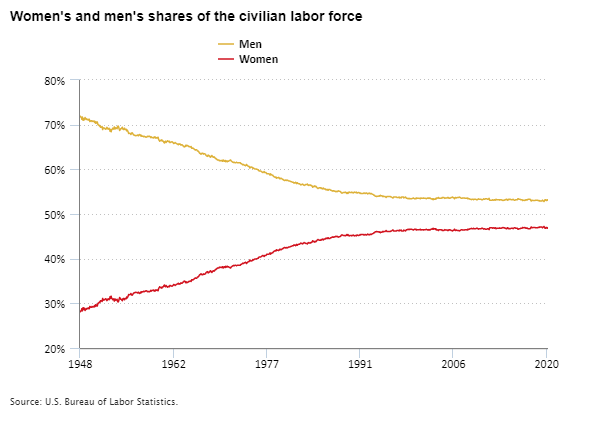
\includegraphics[width=0.7\linewidth]{files/women-73c868b7c60b99ec32c4060e9621d3c8.png}

Following the flattening of the labor force in the 1990s, the 2000s saw a decline, however that was not universal among all demographics. While rates fell for teenagers and young adults, rates increased for men and women over 55 (U.S. Bureau of Labor Statistics, 2016).\footnote{U.S. Bureau of Labor Statistics. (2016, September). Labor force participation: What has happened since the peak? Monthly Labor Review. \href{https://www.bls.gov/opub/mlr/2016/article/labor-force-participation-what-has-happened-since-the-peak.htm}{https://www.bls.gov/opub/mlr/2016/article/labor-force-participation-what-has-happened-since-the-peak.htm}}

Political party leadership may be an area of interest to observe as a large part of the reason those over 55 have began entering the workforce is connected to government instituted programs, namely Social Security. This is in addition to factors such as changes to private retirement plans, an aging population, rising health care costs, and increase in educational attainment (Leonesio, Bridges, Gesumaria, \& Del Bene, 2010).\footnote{Leonesio, M. V., Bridges, B., Gesumaria, R., \& Del Bene, L. (2010, August 22--28). The increasing labor force participation of older workers and its effect on the income of the aged. Social Security Bulletin, 72(1), 59--70. \href{https://www.ssa.gov/policy/docs/ssb/v72n1/v72n1p59.html}{https://www.ssa.gov/policy/docs/ssb/v72n1/v72n1p59.html}}

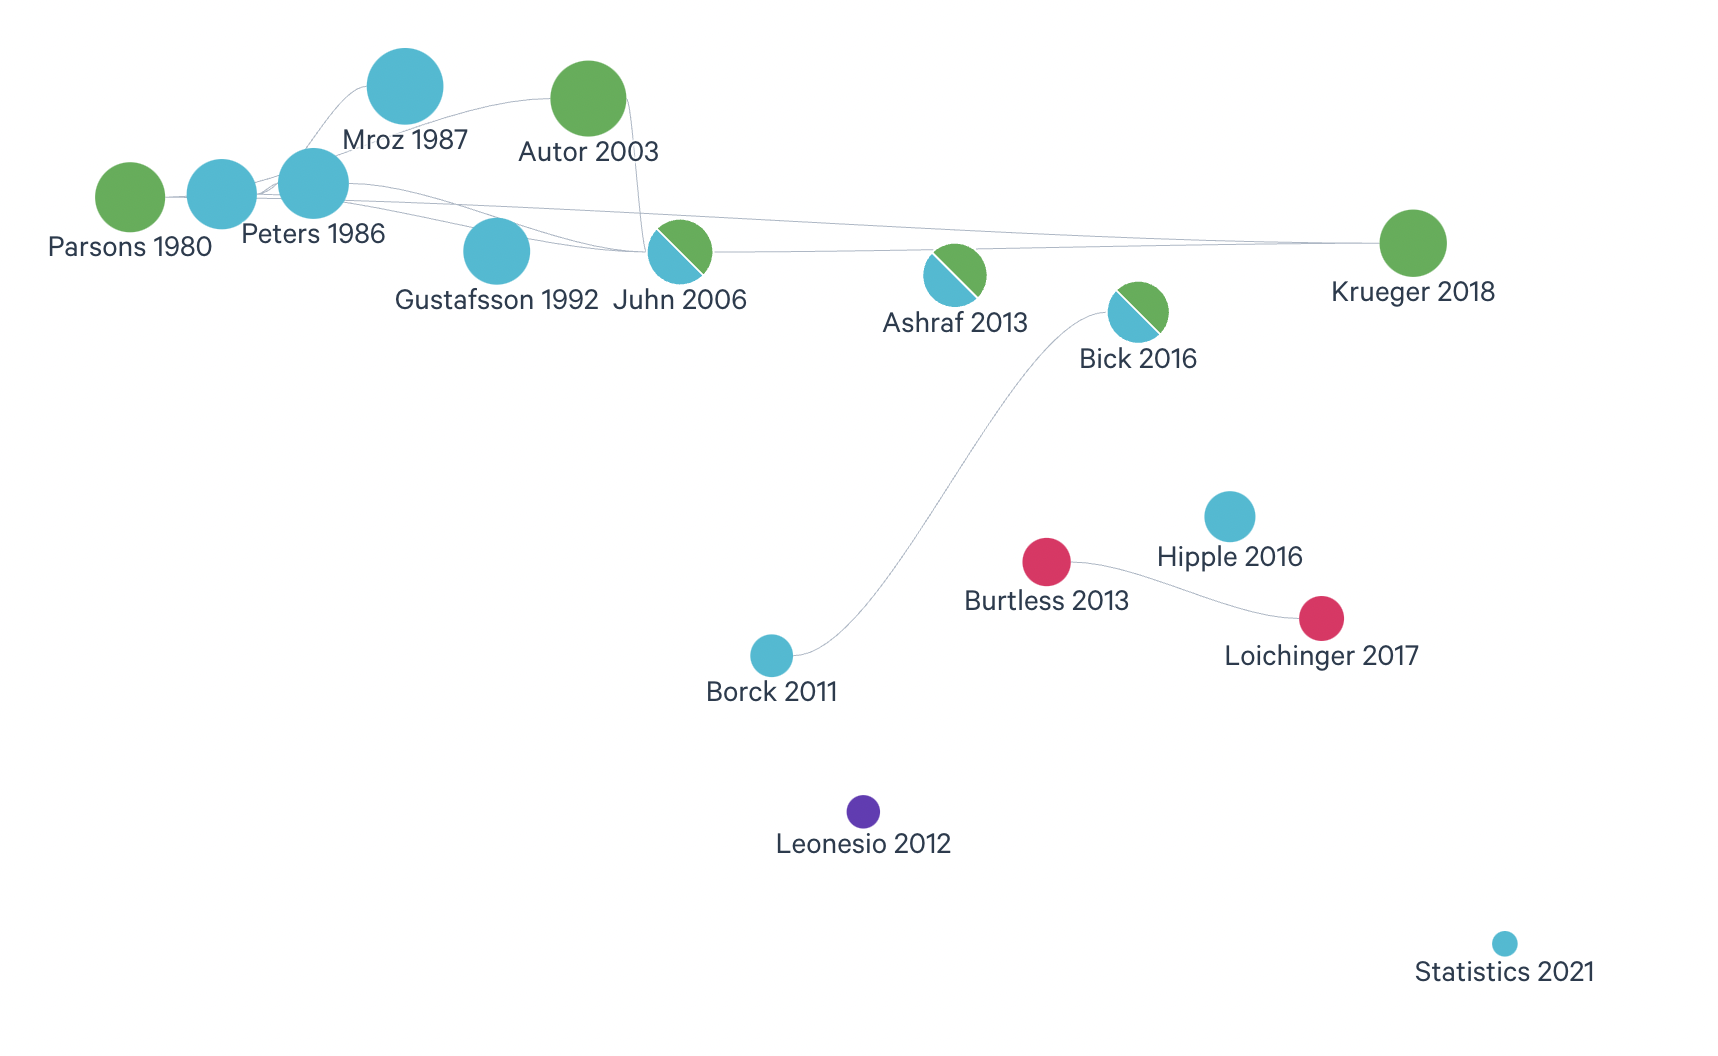
\includegraphics[width=0.7\linewidth]{files/litmap-ba9102f2e95757a03bd4124d2527438a.png}

Access Litmap here\footnote{\href{https://app.litmaps.com/shared/27382733-b5c6-486d-a482-e2b972a348ed}{https://app.litmaps.com/shared/27382733-b5c6-486d-a482-e2b972a348ed}}

\chapter{Methodology}

This study employs a quantitative approach to analyze labor force participation rates across all 50 U.S. states from 1976 to 2020. Data on labor force participation rates were sourced from The Federal Reserve Bank of St. Louis Fed\footnote{Federal Reserve Bank of St. Louis. (n.d.). Civilian labor force participation rate [CIVPART]. Federal Reserve Bank of St. Louis. Retrieved November 11, 2024, from \href{https://fred.stlouisfed.org/series/CIVPART}{https://fred.stlouisfed.org/series/CIVPART}}, while information regarding the political affiliation of each state's governor during this period was compiled into a binary variable, where 1 indicates a Democratic governor and 0 indicates a Republican governor, with the data obtained from Open ICPSR. Additionally, population figures for each state, essential for calculating weighted participation rates, were retrieved from The United States Census Bureau. To compute the weighted labor force participation rates, the study utilized the formula:

\begin{equation}
\text{Weighted Mean} = \frac{\sum (\text{Participation Rate} \times \text{Population})}{\sum \text{Population}}
\end{equation}

As well as a model of the regression analysis:
\begin{equation}

\text{Labor Force Participation Rate} = \beta_0 + \beta_1 \times \text{Democratic Governor} + \epsilon
\end{equation}

To conduct the regression analysis, Python was employed, utilizing libraries such as \texttt{pandas} and \texttt{statsmodels}. The weighted least squares (WLS) method was applied to account for population size, with rigorous checks for linearity, independence, homoscedasticity, and normality of residuals. This methodology provides a comprehensive framework to assess the impact of political governance on labor force participation across the states, facilitating a nuanced understanding of the relationship between governance and workforce engagement.

\textbf{Labor Force Participation Rate (national) Data -- from FRED}

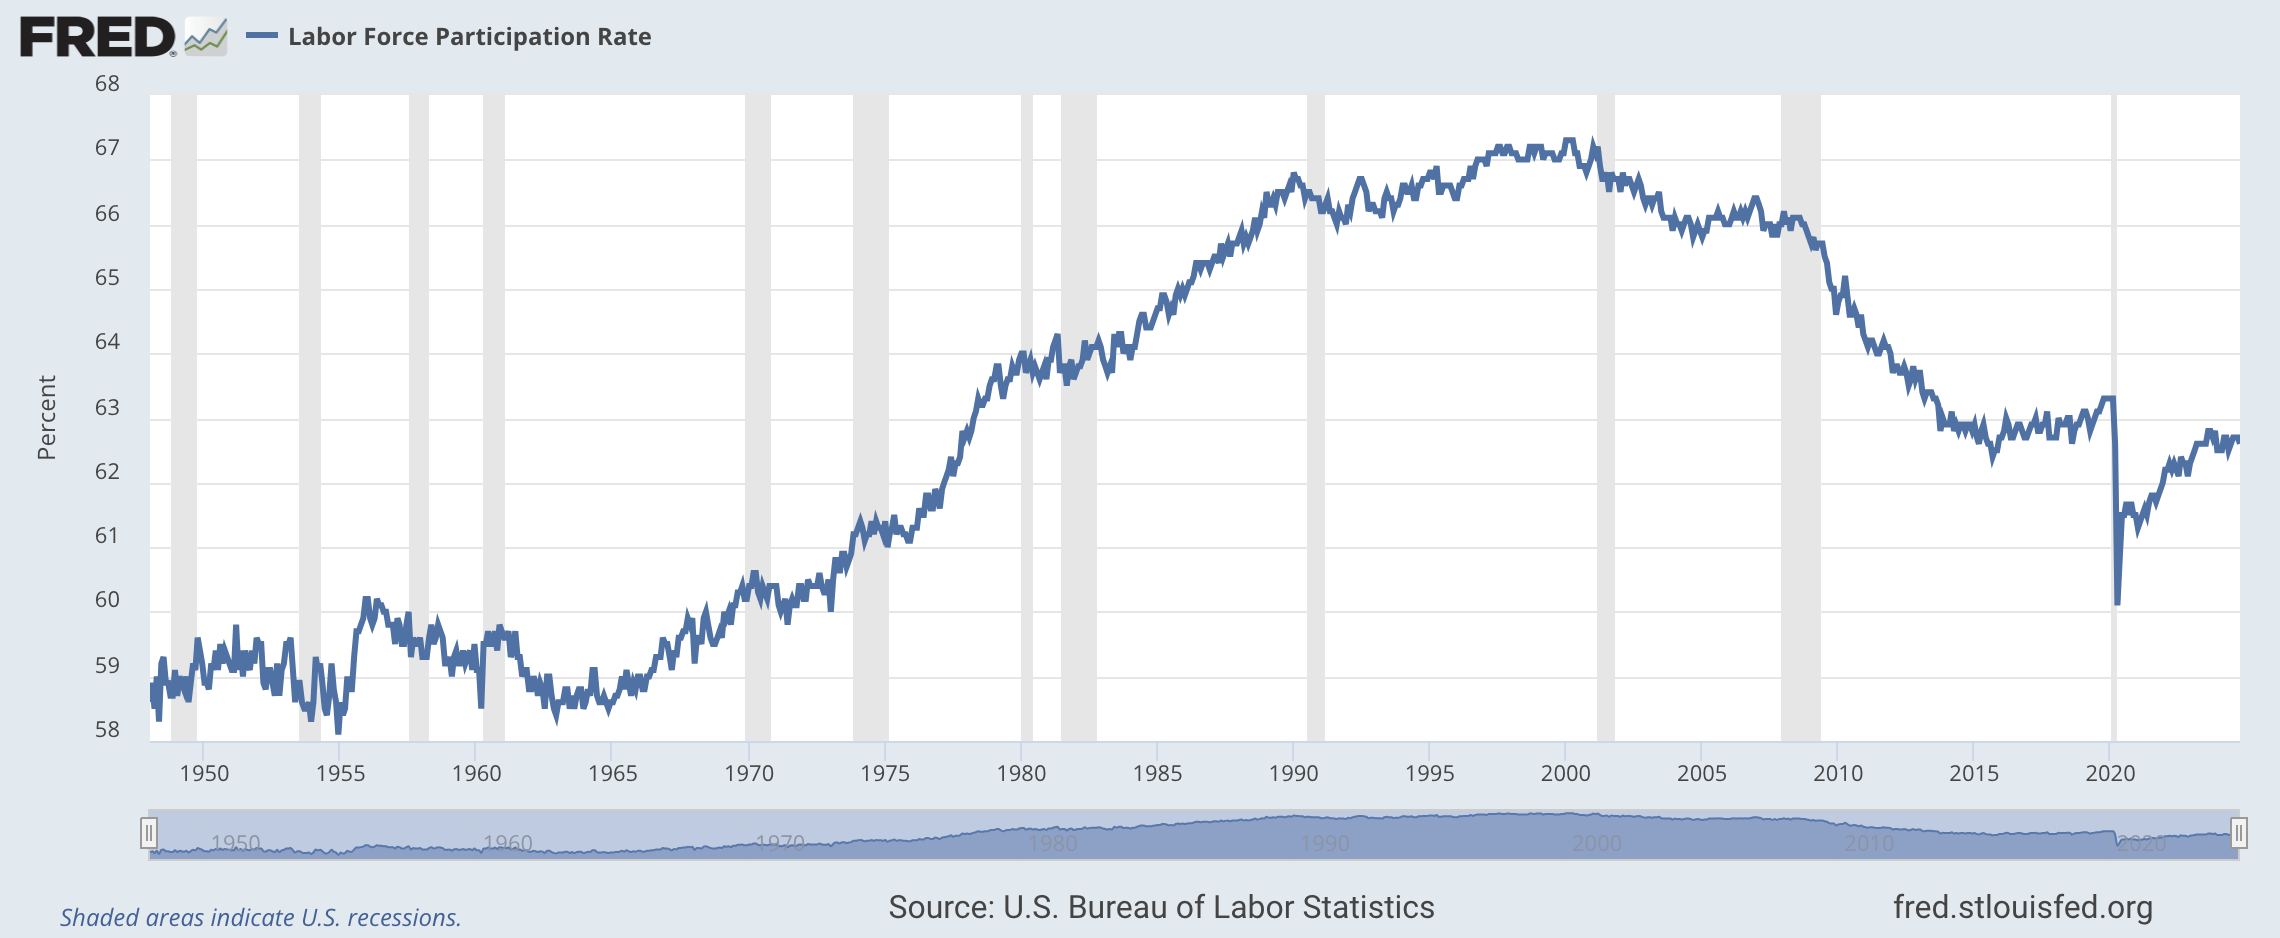
\includegraphics[width=0.7\linewidth]{files/FRED-b4c4bb880b38d58a7677f8cacc531c46.png}

\textbf{Weighted Mean Calculations}

\begin{verbatim}
import pandas as pd

# Load data from a CSV file
df = pd.read_csv('/home/idies/workspace/Temporary/ymettawa/scratch/as.180.369/contrib/yazzymettawa/Paper_Final/Data/stateLFPR.csv')  # Replace 'data.csv' with your actual file path

# Calculate weighted mean for each party
weighted_means = (
    df.assign(Weighted_Participation=df['number'] * df['population'])
    .groupby('party')
    .agg(Weighted_Mean=('Weighted_Participation', 'sum'),
         Total_Population=('population', 'sum'))
    .reset_index()
)

# Calculate final weighted mean
weighted_means['Weighted_Mean'] = weighted_means['Weighted_Mean'] / weighted_means['Total_Population']

# Map party numbers to names
weighted_means['party'] = weighted_means['party'].map({0: 'Republican', 1: 'Democratic'})
# Drop unnecessary columns
weighted_means = weighted_means[['party', 'Weighted_Mean']]

# Print the results
print(weighted_means)
\end{verbatim}

\begin{verbatim}
party  Weighted_Mean
0  Republican      65.486649
1  Democratic      65.188772
\end{verbatim}

\textbf{State Level WLS Regression}

\begin{verbatim}
import pandas as pd
import statsmodels.api as sm
import warnings

# Load data from a CSV file
df = pd.read_csv('/home/idies/workspace/Temporary/ymettawa/scratch/as.180.369/contrib/yazzymettawa/Paper_Final/Data/stateLFPR.csv')  # Replace 'data.csv' with your actual file path

# Define the dependent variable (Y) and independent variable (X)
Y = df['number']
X = df['party']  # Use the Party as a binary variable for regression

# Add a constant to the model
X = sm.add_constant(X)

# Fit the weighted regression model
weights = df['population']  # Use population as weights

# Check for the number of observations
if len(df) >= 8:
    model = sm.WLS(Y, X, weights=weights).fit()
    print(model.summary())
else:
    with warnings.catch_warnings():
        warnings.simplefilter("ignore")
        model = sm.WLS(Y, X, weights=weights).fit()
        print(model.summary())
\end{verbatim}

\begin{verbatim}
WLS Regression Results                            
==============================================================================
Dep. Variable:                 number   R -squared:                       0.002
Model:                            WLS   Adj. R -squared:                  0.001
Method:                 Least Squares   F -statistic:                     3.544
Date:                Mon, 18 Nov 2024   Prob (F -statistic):             0.0599
Time:                        14:13:12   Log -Likelihood:                -5336.4
No. Observations:                1839   AIC:                         1.068e+04
Df Residuals:                    1837   BIC:                         1.069e+04
Df Model:                           1                                         
Covariance Type:            nonrobust                                         
==============================================================================
                 coef    std err          t      P>|t|      [0.025      0.975]
 - - - - - - - - - - - - - - - - - - - - - - - - - - - - - - - - - - - - - - - - - - - - - - - - - - - - - - - - - - - - - - - - - - - - - - - - - - - - - -
const         65.4866      0.109    602.302      0.000      65.273      65.700
party         -0.2979      0.158     -1.882      0.060      -0.608       0.012
==============================================================================
Omnibus:                      231.480   Durbin -Watson:                   1.596
Prob(Omnibus):                  0.000   Jarque -Bera (JB):              370.087
Skew:                          -0.865   Prob(JB):                     4.33e -81
Kurtosis:                       4.356   Cond. No.                         2.56
==============================================================================

Notes:
[1] Standard Errors assume that the covariance matrix of the errors is correctly specified.
\end{verbatim}

\textbf{Interpretting the Results}
Examine the coefficents
\begin{equation}

\beta_1 \text{> 0 = states with Democratic governors have higher LFPR}
\end{equation}

\begin{equation}
\beta_1 \text{< 0 = states with Democratic governors have lower LFPR}
\end{equation}

Statistical Significance: Look at the p-values associated with your coefficients to determine if the results are statistically significant (typically, p \textless  0.05).
Model Fit: Check the R-squared value to see how much of the variance in labor force participation is explained by your model.

\textbf{National Level OLS Regression}

\begin{verbatim}
import pandas as pd
import statsmodels.api as sm

def ols_regression(csv_file):
    # Load the CSV file into a DataFrame
    df = pd.read_csv(csv_file)

    # Extract the necessary columns: 'CIVPART' and 'Party'
    X = df.iloc[:, 4]  # Party column (5th column)
    y = df.iloc[:, 1]  # CIVPART column (2nd column)

    # Add a constant to the model for the intercept term
    X = sm.add_constant(X)

    # Fit the OLS regression model
    model = sm.OLS(y, X).fit()

    # Print the summary of the regression results
    print(model.summary())

# Example usage:
ols_regression('/home/idies/workspace/Temporary/ymettawa/scratch/as.180.369/contrib/yazzymettawa/Paper_Final/Data/nationalLFPR.csv')
\end{verbatim}

\begin{verbatim}
OLS Regression Results                            
==============================================================================
Dep. Variable:                CIVPART   R -squared:                       0.000
Model:                            OLS   Adj. R -squared:                 -0.001
Method:                 Least Squares   F -statistic:                    0.1830
Date:                Mon, 18 Nov 2024   Prob (F -statistic):              0.669
Time:                        14:13:12   Log -Likelihood:                -2023.5
No. Observations:                 816   AIC:                             4051.
Df Residuals:                     814   BIC:                             4060.
Df Model:                           1                                         
Covariance Type:            nonrobust                                         
==============================================================================
                 coef    std err          t      P>|t|      [0.025      0.975]
 - - - - - - - - - - - - - - - - - - - - - - - - - - - - - - - - - - - - - - - - - - - - - - - - - - - - - - - - - - - - - - - - - - - - - - - - - - - - - -
const         63.1123      0.132    478.078      0.000      62.853      63.371
Party          0.0880      0.206      0.428      0.669      -0.316       0.492
==============================================================================
Omnibus:                    10216.381   Durbin -Watson:                   0.005
Prob(Omnibus):                  0.000   Jarque -Bera (JB):               72.909
Skew:                          -0.184   Prob(JB):                     1.47e -16
Kurtosis:                       1.583   Cond. No.                         2.46
==============================================================================

Notes:
[1] Standard Errors assume that the covariance matrix of the errors is correctly specified.
\end{verbatim}

\section{Results}

Returning to the research question: ``How does the labor force participation rate from the 1953 until 2020 in the United States vary with political party governance" the results suggest that there is little evidence to support a strong or reliable relationship between political party governance and labor force participation rates. This was found to be the case when observing both national political party governance (through the president's party affiliation and state labor force participation rates) as well on the state level (through the governor's party affiliation and state labor force participation rates). However, on the state level the tendency was for participation rates to be higher during Democrat governorships, while on the national level the tendency was for participation rates to be higher during Republican presidencies further undermining any relationship.

\textbf{State Level}

The WLS regression results indicate a  weak relationship between the independent variable (party) and the dependent variable (labor force participation rate). The effect of ``party'' is marginally statistically significant (p $\approx$ 0.06), but the overall model fit is very poor (R\textsuperscript{2} $\approx$ 0.002). The low R-squared value indicates that the predictor ``party'' explains almost none of the variance in ``number.''

\begin{equation}
\text{STATE CIVPART} = 65.4866 + -0.2979 \times \text{Party}
\end{equation}

\textbf{National Level}

The OLS regression results indicate a  weak relationship between the independent variable (party) and the dependent variable (labor force participation rate). The effect of ``party'' is marginally statistically significant (p $\approx$ 0.669), but the overall model fit is very poor (with an adjusted R\textsuperscript{2} $\approx$ -0.001). The low R-squared value indicates that the predictor ``party'' explains almost none of the variance in ``number.''

\begin{equation}
\text{NATIONAL CIVPART} = 63.1123 + 0.0880 \times \text{Party}
\end{equation}

\chapter{Conclusion}

In this paper, the question of how the labor force participation rate from 1948 until 2020 in the United States varied with political party governance was explored. The findings are that both the state level, as determined by the governor's political party affiliation, and the national level, as determined by the president's political party affiliation, had no statistically significant correlation with the labor force participation rate of the state or country. Further research into other branches of government and political affiliations, both local and in the House of Representatives can be used to further describe the existence or non-existence of a relationship. Some limitations include the limited time scope due to data constraints, as well as the lack of statistical accounting for economic and social factors affecting labor force participation rates outside of preliminary research. In terms of broader implications, specific policies, and their effects would need to be observed as opposed to the general policies of each political party to determine their effectiveness.

\chapter{Bibliography}

\begin{verbatim}
import bibtexparser

# Open and load the .bib file
with open('newreferences.bib') as bibfile:
    bib_database = bibtexparser.load(bibfile)

# Function to format each entry in APA style
def format_apa(entry):
    authors = entry.get('author', '').replace(',', '').split(' and ')
    authors = [author.strip() for author in authors]  # Clean up the authors' names

    # Format authors in APA style (last name, first initial)
    formatted_authors = ', '.join([f"{name.split(' ')[ -1]}, {' '.join(name.split(' ')[: -1])[:1]}." for name in authors])
    
    # Handle publication year
    year = entry.get('year', 'n.d.')  # Use 'n.d.' for no date
    
    # Title of the article
    title = entry.get('title', '')
    
    # Journal details (if applicable)
    journal = entry.get('journal', '')
    volume = entry.get('volume', '')
    issue = entry.get('number', '')
    pages = entry.get('pages', '')
    
    # Build the APA formatted citation
    citation = f"{formatted_authors} ({year}). {title}. {journal}, {volume}({issue}), {pages}."
    
    # If there is no journal, it's likely a book or other type of source.
    if not journal:
        publisher = entry.get('publisher', 'Publisher not available')
        citation = f"{formatted_authors} ({year}). {title}. {publisher}."
    
    return citation

# Print each reference in APA format
for entry in bib_database.entries:
    citation = format_apa(entry)
    print(citation)
    print("\n")  # Separate citations by a newline
\end{verbatim}

\begin{verbatim}
Rainald, B. (2011). Adieu rabenmutter - the effect of culture on fertility, female
labour supply, the gender wage gap and childcare. SSRN Electron. J., (), .


B, K. (2017). Where have all the workers gone? An inquiry into the decline of
the {U}.s. labor force participation rate. Brookings Pap. Econ. Act., 2017(2), 1 - -87.


Gary, B. (2013). Can Educational Attainment Explain the Rise in Labor Force
Participation at Older Ages?. Center for Retirement Research.


Rainald, B. (n.d.). ``Adieu Rabenmutter''—culture, fertility, female labour supply, the
gender wage gap and childcare. J. Popul. Econ., (), .


H, A., N, W., Joshua, W. (2013). The effect of fertility reduction on economic growth. Popul. Dev. Rev., 39(1), 97 - -130.


R, J., Jonathan, S. (n.d.). Labor Supply and Marital Separation. Publisher not available.


Chinhui, J., M, P. (2006). Changes in labor force participation in the United States. Journal of Economic Perspectives, 20(3), 27 - -46.


Elke, L., Alexia, P. (2017). Changes in economic activity: The role of age and education. Demogr. Res., 36(), 1185 - -1208.


And, F. (n.d.). {THE} {QUANTITATIVE} {ROLE} {OF} {CHILD} {CARE} {FOR} {FEMALE}
{LABOR} {FORCE} {PARTICIPATION}. Publisher not available.


Siv, G., Frank, S. (1992). Child care subsidies and labor supply in Sweden. J. Hum. Resour., 27(1), 204.


H, A., G, D. (2003). The rise in the disability rolls and the decline in unemployment. Q. J. Econ., 118(1), 157 - -206.


B, K. (2017). Where Have All the Workers Gone. Brookings Papers on Economic Activity, (Fall 2017), .


O, P. (1980). The decline in male labor force participation. J. Polit. Econ., 88(1), 117 - -134.
\end{verbatim}

\chapter{Appendix}

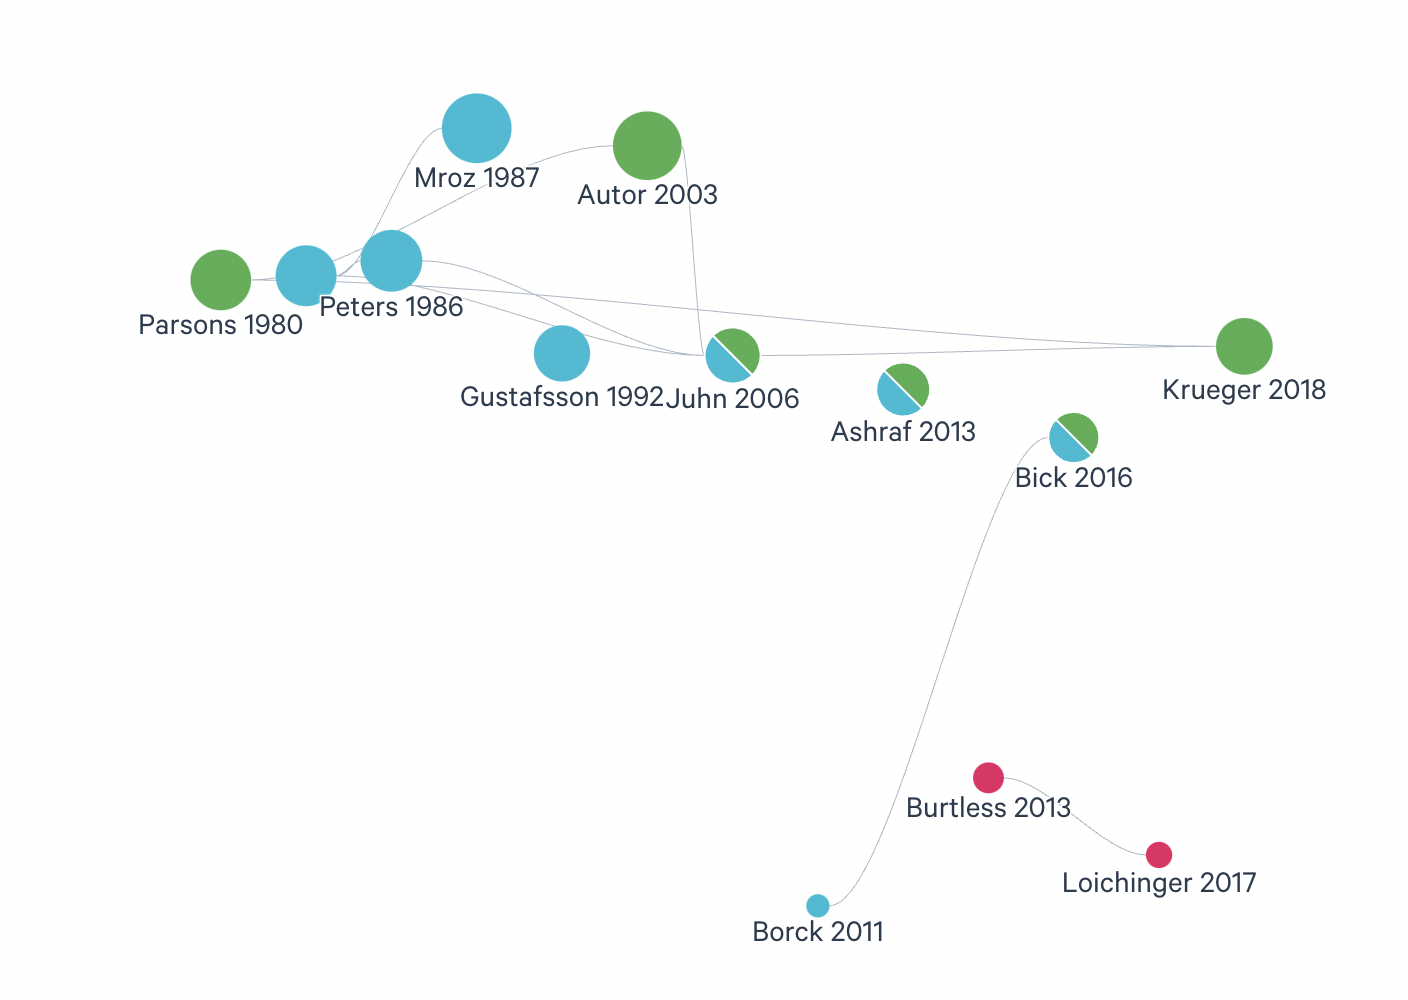
\includegraphics[width=0.7\linewidth]{files/litmap-8f985aea6f5acab8c2e3bdc1dbe2eff7.png}

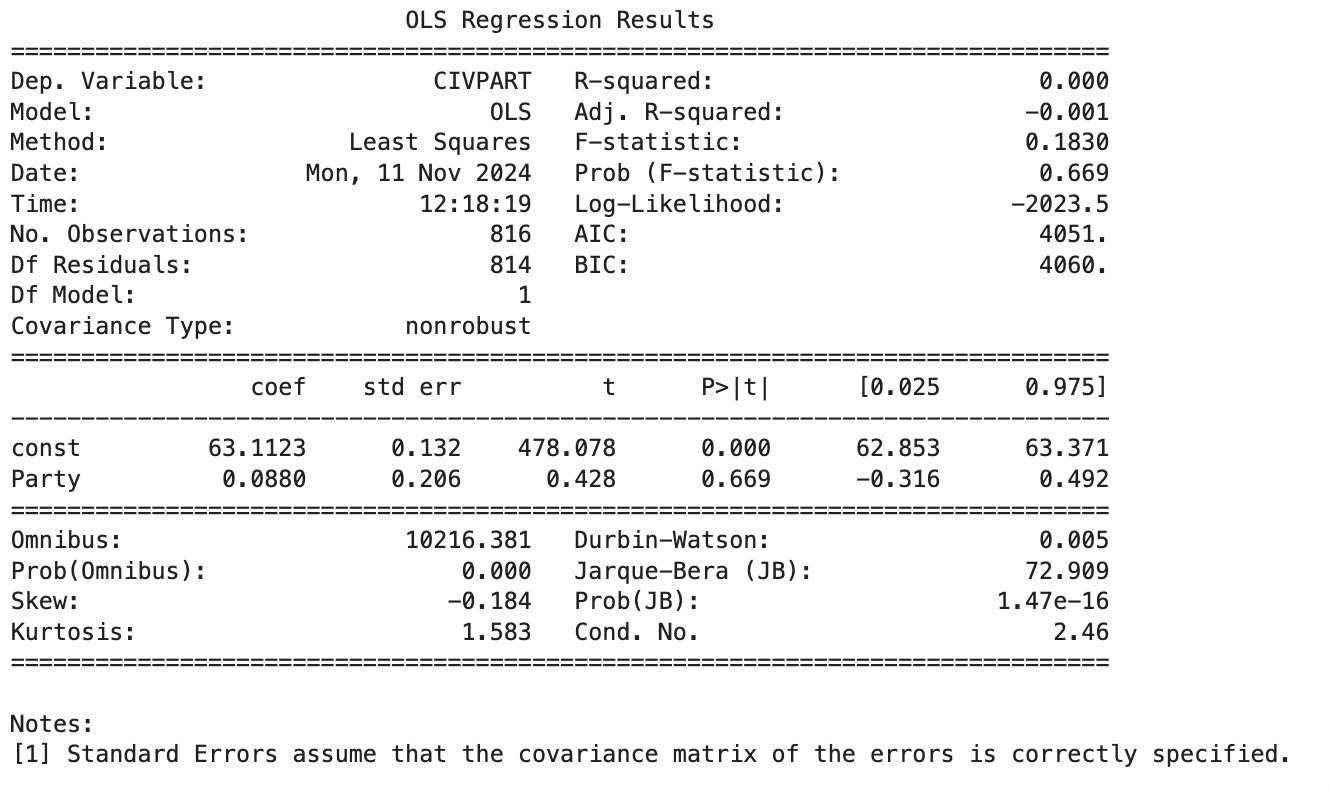
\includegraphics[width=0.7\linewidth]{files/OLS-c5cf87287ef4675b97d7a4a27f7664a6.png}

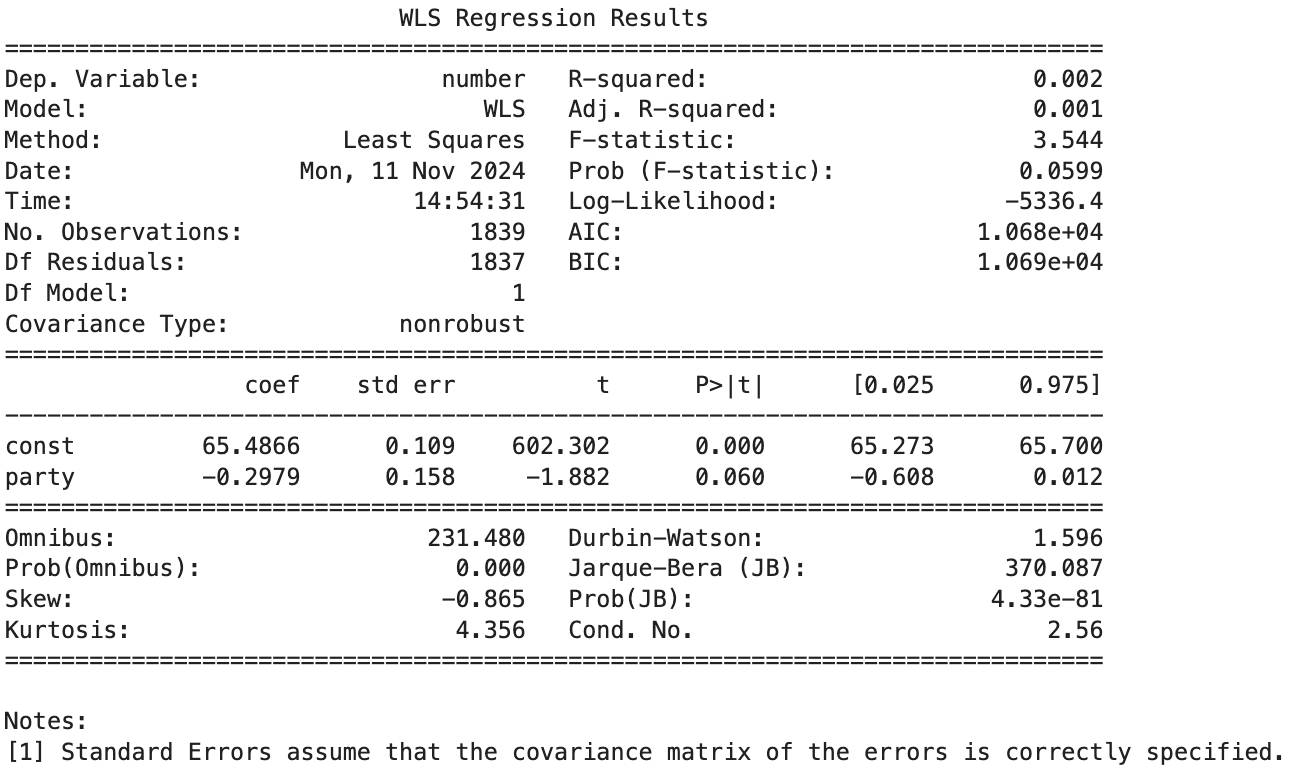
\includegraphics[width=0.7\linewidth]{files/WLS-c513dc796a7e1b69f6856fefaa83e78e.png}





\bibliographystyle{unsrtnat}
\bibliography{main.bib}

\end{document}
